
%% bare_conf.tex
%% V1.4b
%% 2015/08/26
%% by Michael Shell
%% See:
%% http://www.michaelshell.org/
%% for current contact information.
%%
%% This is a skeleton file demonstrating the use of IEEEtran.cls
%% (requires IEEEtran.cls version 1.8b or later) with an IEEE
%% conference paper.
%%
%% Support sites:
%% http://www.michaelshell.org/tex/ieeetran/
%% http://www.ctan.org/pkg/ieeetran
%% and
%% http://www.ieee.org/

%%*************************************************************************
%% Legal Notice:
%% This code is offered as-is without any warranty either expressed or
%% implied; without even the implied warranty of MERCHANTABILITY or
%% FITNESS FOR A PARTICULAR PURPOSE! 
%% User assumes all risk.
%% In no event shall the IEEE or any contributor to this code be liable for
%% any damages or losses, including, but not limited to, incidental,
%% consequential, or any other damages, resulting from the use or misuse
%% of any information contained here.
%%
%% All comments are the opinions of their respective authors and are not
%% necessarily endorsed by the IEEE.
%%
%% This work is distributed under the LaTeX Project Public License (LPPL)
%% ( http://www.latex-project.org/ ) version 1.3, and may be freely used,
%% distributed and modified. A copy of the LPPL, version 1.3, is included
%% in the base LaTeX documentation of all distributions of LaTeX released
%% 2003/12/01 or later.
%% Retain all contribution notices and credits.
%% ** Modified files should be clearly indicated as such, including  **
%% ** renaming them and changing author support contact information. **
%%*************************************************************************


% *** Authors should verify (and, if needed, correct) their LaTeX system  ***
% *** with the testflow diagnostic prior to trusting their LaTeX platform ***
% *** with production work. The IEEE's font choices and paper sizes can   ***
% *** trigger bugs that do not appear when using other class files.       ***                          ***
% The testflow support page is at:
% http://www.michaelshell.org/tex/testflow/



\documentclass[conference]{IEEEtran}
% Some Computer Society conferences also require the compsoc mode option,
% but others use the standard conference format.
%
% If IEEEtran.cls has not been installed into the LaTeX system files,
% manually specify the path to it like:
% \documentclass[conference]{../sty/IEEEtran}





% Some very useful LaTeX packages include:
% (uncomment the ones you want to load)


% *** MISC UTILITY PACKAGES ***
%
%\usepackage{ifpdf}
% Heiko Oberdiek's ifpdf.sty is very useful if you need conditional
% compilation based on whether the output is pdf or dvi.
% usage:
% \ifpdf
%   % pdf code
% \else
%   % dvi code
% \fi
% The latest version of ifpdf.sty can be obtained from:
% http://www.ctan.org/pkg/ifpdf
% Also, note that IEEEtran.cls V1.7 and later provides a builtin
% \ifCLASSINFOpdf conditional that works the same way.
% When switching from latex to pdflatex and vice-versa, the compiler may
% have to be run twice to clear warning/error messages.






% *** CITATION PACKAGES ***
%
%\usepackage{cite}
% cite.sty was written by Donald Arseneau
% V1.6 and later of IEEEtran pre-defines the format of the cite.sty package
% \cite{} output to follow that of the IEEE. Loading the cite package will
% result in citation numbers being automatically sorted and properly
% "compressed/ranged". e.g., [1], [9], [2], [7], [5], [6] without using
% cite.sty will become [1], [2], [5]--[7], [9] using cite.sty. cite.sty's
% \cite will automatically add leading space, if needed. Use cite.sty's
% noadjust option (cite.sty V3.8 and later) if you want to turn this off
% such as if a citation ever needs to be enclosed in parenthesis.
% cite.sty is already installed on most LaTeX systems. Be sure and use
% version 5.0 (2009-03-20) and later if using hyperref.sty.
% The latest version can be obtained at:
% http://www.ctan.org/pkg/cite
% The documentation is contained in the cite.sty file itself.






% *** GRAPHICS RELATED PACKAGES ***
%
\ifCLASSINFOpdf
\usepackage[pdftex]{graphicx}
  % declare the path(s) where your graphic files are
 \graphicspath{{images/}}
  % and their extensions so you won't have to specify these with
  % every instance of \includegraphics
 \DeclareGraphicsExtensions{.pdf,.jpeg,.png}
\else
  % or other class option (dvipsone, dvipdf, if not using dvips). graphicx
  % will default to the driver specified in the system graphics.cfg if no
  % driver is specified.
  % \usepackage[dvips]{graphicx}
  % declare the path(s) where your graphic files are
  % \graphicspath{{../eps/}}
  % and their extensions so you won't have to specify these with
  % every instance of \includegraphics
  % \DeclareGraphicsExtensions{.eps}
\fi
% graphicx was written by David Carlisle and Sebastian Rahtz. It is
% required if you want graphics, photos, etc. graphicx.sty is already
% installed on most LaTeX systems. The latest version and documentation
% can be obtained at: 
% http://www.ctan.org/pkg/graphicx
% Another good source of documentation is "Using Imported Graphics in
% LaTeX2e" by Keith Reckdahl which can be found at:
% http://www.ctan.org/pkg/epslatex
%
% latex, and pdflatex in dvi mode, support graphics in encapsulated
% postscript (.eps) format. pdflatex in pdf mode supports graphics
% in .pdf, .jpeg, .png and .mps (metapost) formats. Users should ensure
% that all non-photo figures use a vector format (.eps, .pdf, .mps) and
% not a bitmapped formats (.jpeg, .png). The IEEE frowns on bitmapped formats
% which can result in "jaggedy"/blurry rendering of lines and letters as
% well as large increases in file sizes.
%
% You can find documentation about the pdfTeX application at:
% http://www.tug.org/applications/pdftex





% *** MATH PACKAGES ***
%
%\usepackage{amsmath}
% A popular package from the American Mathematical Society that provides
% many useful and powerful commands for dealing with mathematics.
%
% Note that the amsmath package sets \interdisplaylinepenalty to 10000
% thus preventing page breaks from occurring within multiline equations. Use:
%\interdisplaylinepenalty=2500
% after loading amsmath to restore such page breaks as IEEEtran.cls normally
% does. amsmath.sty is already installed on most LaTeX systems. The latest
% version and documentation can be obtained at:
% http://www.ctan.org/pkg/amsmath





% *** SPECIALIZED LIST PACKAGES ***
%
%\usepackage{algorithmic}
% algorithmic.sty was written by Peter Williams and Rogerio Brito.
% This package provides an algorithmic environment fo describing algorithms.
% You can use the algorithmic environment in-text or within a figure
% environment to provide for a floating algorithm. Do NOT use the algorithm
% floating environment provided by algorithm.sty (by the same authors) or
% algorithm2e.sty (by Christophe Fiorio) as the IEEE does not use dedicated
% algorithm float types and packages that provide these will not provide
% correct IEEE style captions. The latest version and documentation of
% algorithmic.sty can be obtained at:
% http://www.ctan.org/pkg/algorithms
% Also of interest may be the (relatively newer and more customizable)
% algorithmicx.sty package by Szasz Janos:
% http://www.ctan.org/pkg/algorithmicx




% *** ALIGNMENT PACKAGES ***
%
%\usepackage{array}
% Frank Mittelbach's and David Carlisle's array.sty patches and improves
% the standard LaTeX2e array and tabular environments to provide better
% appearance and additional user controls. As the default LaTeX2e table
% generation code is lacking to the point of almost being broken with
% respect to the quality of the end results, all users are strongly
% advised to use an enhanced (at the very least that provided by array.sty)
% set of table tools. array.sty is already installed on most systems. The
% latest version and documentation can be obtained at:
% http://www.ctan.org/pkg/array


% IEEEtran contains the IEEEeqnarray family of commands that can be used to
% generate multiline equations as well as matrices, tables, etc., of high
% quality.




% *** SUBFIGURE PACKAGES ***
%\ifCLASSOPTIONcompsoc
%  \usepackage[caption=false,font=normalsize,labelfont=sf,textfont=sf]{subfig}
%\else
%  \usepackage[caption=false,font=footnotesize]{subfig}
%\fi
% subfig.sty, written by Steven Douglas Cochran, is the modern replacement
% for subfigure.sty, the latter of which is no longer maintained and is
% incompatible with some LaTeX packages including fixltx2e. However,
% subfig.sty requires and automatically loads Axel Sommerfeldt's caption.sty
% which will override IEEEtran.cls' handling of captions and this will result
% in non-IEEE style figure/table captions. To prevent this problem, be sure
% and invoke subfig.sty's "caption=false" package option (available since
% subfig.sty version 1.3, 2005/06/28) as this is will preserve IEEEtran.cls
% handling of captions.
% Note that the Computer Society format requires a larger sans serif font
% than the serif footnote size font used in traditional IEEE formatting
% and thus the need to invoke different subfig.sty package options depending
% on whether compsoc mode has been enabled.
%
% The latest version and documentation of subfig.sty can be obtained at:
% http://www.ctan.org/pkg/subfig




% *** FLOAT PACKAGES ***
%
%\usepackage{fixltx2e}
% fixltx2e, the successor to the earlier fix2col.sty, was written by
% Frank Mittelbach and David Carlisle. This package corrects a few problems
% in the LaTeX2e kernel, the most notable of which is that in current
% LaTeX2e releases, the ordering of single and double column floats is not
% guaranteed to be preserved. Thus, an unpatched LaTeX2e can allow a
% single column figure to be placed prior to an earlier double column
% figure.
% Be aware that LaTeX2e kernels dated 2015 and later have fixltx2e.sty's
% corrections already built into the system in which case a warning will
% be issued if an attempt is made to load fixltx2e.sty as it is no longer
% needed.
% The latest version and documentation can be found at:
% http://www.ctan.org/pkg/fixltx2e


%\usepackage{stfloats}
% stfloats.sty was written by Sigitas Tolusis. This package gives LaTeX2e
% the ability to do double column floats at the bottom of the page as well
% as the top. (e.g., "\begin{figure*}[!b]" is not normally possible in
% LaTeX2e). It also provides a command:
%\fnbelowfloat
% to enable the placement of footnotes below bottom floats (the standard
% LaTeX2e kernel puts them above bottom floats). This is an invasive package
% which rewrites many portions of the LaTeX2e float routines. It may not work
% with other packages that modify the LaTeX2e float routines. The latest
% version and documentation can be obtained at:
% http://www.ctan.org/pkg/stfloats
% Do not use the stfloats baselinefloat ability as the IEEE does not allow
% \baselineskip to stretch. Authors submitting work to the IEEE should note
% that the IEEE rarely uses double column equations and that authors should try
% to avoid such use. Do not be tempted to use the cuted.sty or midfloat.sty
% packages (also by Sigitas Tolusis) as the IEEE does not format its papers in
% such ways.
% Do not attempt to use stfloats with fixltx2e as they are incompatible.
% Instead, use Morten Hogholm'a dblfloatfix which combines the features
% of both fixltx2e and stfloats:
%
% \usepackage{dblfloatfix}
% The latest version can be found at:
% http://www.ctan.org/pkg/dblfloatfix




% *** PDF, URL AND HYPERLINK PACKAGES ***
%
%\usepackage{url}
% url.sty was written by Donald Arseneau. It provides better support for
% handling and breaking URLs. url.sty is already installed on most LaTeX
% systems. The latest version and documentation can be obtained at:
% http://www.ctan.org/pkg/url
% Basically, \url{my_url_here}.




% *** Do not adjust lengths that control margins, column widths, etc. ***
% *** Do not use packages that alter fonts (such as pslatex).         ***
% There should be no need to do such things with IEEEtran.cls V1.6 and later.
% (Unless specifically asked to do so by the journal or conference you plan
% to submit to, of course. )


% correct bad hyphenation here
\hyphenation{op-tical net-works semi-conduc-tor}


\begin{document}
%
% paper title
% Titles are generally capitalized except for words such as a, an, and, as,
% at, but, by, for, in, nor, of, on, or, the, to and up, which are usually
% not capitalized unless they are the first or last word of the title.
% Linebreaks \\ can be used within to get better formatting as desired.
% Do not put math or special symbols in the title.
\title{Learning the McGurk Effect\\ from Raw Input}


% author names and affiliations
% use a multiple column layout for up to three different
% affiliations
\author{\IEEEauthorblockN{Darryl Hannan}
\IEEEauthorblockA{Villanova University\\
Email: dhannan1@villanova.edu}
}

% conference papers do not typically use \thanks and this command
% is locked out in conference mode. If really needed, such as for
% the acknowledgment of grants, issue a \IEEEoverridecommandlockouts
% after \documentclass

% for over three affiliations, or if they all won't fit within the width
% of the page, use this alternative format:
% 
%\author{\IEEEauthorblockN{Michael Shell\IEEEauthorrefmark{1},
%Homer Simpson\IEEEauthorrefmark{2},
%James Kirk\IEEEauthorrefmark{3}, 
%Montgomery Scott\IEEEauthorrefmark{3} and
%Eldon Tyrell\IEEEauthorrefmark{4}}
%\IEEEauthorblockA{\IEEEauthorrefmark{1}School of Electrical and Computer Engineering\\
%Georgia Institute of Technology,
%Atlanta, Georgia 30332--0250\\ Email: see http://www.michaelshell.org/contact.html}
%\IEEEauthorblockA{\IEEEauthorrefmark{2}Twentieth Century Fox, Springfield, USA\\
%Email: homer@thesimpsons.com}
%\IEEEauthorblockA{\IEEEauthorrefmark{3}Starfleet Academy, San Francisco, California 96678-2391\\
%Telephone: (800) 555--1212, Fax: (888) 555--1212}
%\IEEEauthorblockA{\IEEEauthorrefmark{4}Tyrell Inc., 123 Replicant Street, Los Angeles, California 90210--4321}}




% use for special paper notices
%\IEEEspecialpapernotice{(Invited Paper)}




% make the title area
\maketitle

% As a general rule, do not put math, special symbols or citations
% in the abstract
\begin{abstract}
The McGurk effect is a cognitive phenomenon that occurs when individuals attempt to interpret a mismatched phoneme/viseme pair, resulting in the perception of a third sound. This effect is a clear example of multimodal processing in the human brain. Here, I attempt to create a multimodal convolutional neural network that learns a joint embedding space such that the trained model exhibits the McGurk effect. The model was unable to produce the effect due to the nature of the embedding space. However, the results have provided me with some insights regarding potential modifications that can be made to the model.
\end{abstract}

% no keywords




% For peer review papers, you can put extra information on the cover
% page as needed:
% \ifCLASSOPTIONpeerreview
% \begin{center} \bfseries EDICS Category: 3-BBND \end{center}
% \fi
%
% For peerreview papers, this IEEEtran command inserts a page break and
% creates the second title. It will be ignored for other modes.
\IEEEpeerreviewmaketitle



\section{Introduction}
Humans are really good at multimodal processing. Every moment, we are bombarded with a profusion of information from multiple modalities, and manage to assemble it into a unified coherent experience. Machines, on the other hand, can only perform basic multimodal tasks, such as image captioning and visual question answering. Here, I apply multimodal machine learning techniques to auditory and visual information.

The smallest units of language are known as phonemes. Examples of phonemes include the /th/ sound in "the" and the /k/ sound in "cat". English is composed of 44 phonemes, despite having only 26 letters. A viseme is the lip movement associated with a phoneme. This relationship is not one-to-one, with some phonemes sharing visemes. When people are actively engaged in conversation, their interpretation of what the other person is saying is not solely based upon auditory information. So long as they are looking at the person who is speaking, they also rely upon visual information in the form of visemes.

This relationship is demonstrated by the McGurk effect.\cite{McGurk1976} The McGurk effect occurs when the phoneme and viseme do not match. Each modality indicates a different sound to the brain. Unsure how to handle this conflicting information, the brain tends to combine the two sounds. This can result in the perception of a third sound that wasn't expressed in either modality. The classic example of this occurs when the phoneme is /b/a and the viseme is /g/a; many individuals report hearing /d/a.

Here, I construct a convolutional autoencoder that learns the relationship between phonemes and visemes. The model merges each modality into a joint embedding space, and then attempts to reconstruct the inputs. The goal of the project is to learn a joint embedding space that is robust enough for the trained model to exhibit the McGurk effect.
% An example of a floating figure using the graphicx package.
% Note that \label must occur AFTER (or within) \caption.
% For figures, \caption should occur after the \includegraphics.
% Note that IEEEtran v1.7 and later has special internal code that
% is designed to preserve the operation of \label within \caption
% even when the captionsoff option is in effect. However, because
% of issues like this, it may be the safest practice to put all your
% \label just after \caption rather than within \caption{}.
%
% Reminder: the "draftcls" or "draftclsnofoot", not "draft", class
% option should be used if it is desired that the figures are to be
% displayed while in draft mode.
%
%\begin{figure}[!t]
%\centering
%\includegraphics[width=2.5in]{myfigure}
% where an .eps filename suffix will be assumed under latex, 
% and a .pdf suffix will be assumed for pdflatex; or what has been declared
% via \DeclareGraphicsExtensions.
%\caption{Simulation results for the network.}
%\label{fig_sim}
%\end{figure}

% Note that the IEEE typically puts floats only at the top, even when this
% results in a large percentage of a column being occupied by floats.


% An example of a double column floating figure using two subfigures.
% (The subfig.sty package must be loaded for this to work.)
% The subfigure \label commands are set within each subfloat command,
% and the \label for the overall figure must come after \caption.
% \hfil is used as a separator to get equal spacing.
% Watch out that the combined width of all the subfigures on a 
% line do not exceed the text width or a line break will occur.
%
%\begin{figure*}[!t]
%\centering
%\subfloat[Case I]{\includegraphics[width=2.5in]{box}%
%\label{fig_first_case}}
%\hfil
%\subfloat[Case II]{\includegraphics[width=2.5in]{box}%
%\label{fig_second_case}}
%\caption{Simulation results for the network.}
%\label{fig_sim}
%\end{figure*}
%
% Note that often IEEE papers with subfigures do not employ subfigure
% captions (using the optional argument to \subfloat[]), but instead will
% reference/describe all of them (a), (b), etc., within the main caption.
% Be aware that for subfig.sty to generate the (a), (b), etc., subfigure
% labels, the optional argument to \subfloat must be present. If a
% subcaption is not desired, just leave its contents blank,
% e.g., \subfloat[].


% An example of a floating table. Note that, for IEEE style tables, the
% \caption command should come BEFORE the table and, given that table
% captions serve much like titles, are usually capitalized except for words
% such as a, an, and, as, at, but, by, for, in, nor, of, on, or, the, to
% and up, which are usually not capitalized unless they are the first or
% last word of the caption. Table text will default to \footnotesize as
% the IEEE normally uses this smaller font for tables.
% The \label must come after \caption as always.
%
%\begin{table}[!t]
%% increase table row spacing, adjust to taste
%\renewcommand{\arraystretch}{1.3}
% if using array.sty, it might be a good idea to tweak the value of
% \extrarowheight as needed to properly center the text within the cells
%\caption{An Example of a Table}
%\label{table_example}
%\centering
%% Some packages, such as MDW tools, offer better commands for making tables
%% than the plain LaTeX2e tabular which is used here.
%\begin{tabular}{|c||c|}
%\hline
%One & Two\\
%\hline
%Three & Four\\
%\hline
%\end{tabular}
%\end{table}


% Note that the IEEE does not put floats in the very first column
% - or typically anywhere on the first page for that matter. Also,
% in-text middle ("here") positioning is typically not used, but it
% is allowed and encouraged for Computer Society conferences (but
% not Computer Society journals). Most IEEE journals/conferences use
% top floats exclusively. 
% Note that, LaTeX2e, unlike IEEE journals/conferences, places
% footnotes above bottom floats. This can be corrected via the
% \fnbelowfloat command of the stfloats package.

\section{Related Work}
This is not the first attempt at using machine learning to model the McGurk effect. Sporea and Gruning (2010) use an artificial neural network to model the effect.\cite{Sporea2010} This model was created prior to the popularization of convolutional networks. They extract cues from the data, such as mouth width and height, and use these features as input. They also treat the problem as a classification task, where classes are phonemes.

A most recent work, by Getz et al. (2017), uses gaussian mixture models (GMMs) to learn the effect.\cite{Getz2017} They use their model to simulate the developmental process that humans go through to learn phonological categories. The inputs to this model also take the form of extracted cues.

Other models attempt to learn the relationship between auditory and visual information, but do not model the McGurk effect. Current state of the art is seen in the work of Torfi et al. (2017).\cite{Torfi2017} They use a 3D convolutional autoencoder to handle both the spatial and temporal natures of the visual information. Features are extracted from the auditory information and fed into the model as vectors.

A major component of my model is that it uses raw input. The visual modality is represented using video frames and the audio modality is represented using a raw waveform. This complicates things for the model, requiring it to extract both spatial and temporal information, but it limits preprocessing and allows the model to determine which cues to extract.

\section{Methodolgy}
\subsection{The Data}
The data is obtained from the GRID audio-visual sentence corpus.\cite{Cooke2006} This dataset consists of videos of 34 individuals reading sentences 1000 sentences aloud. Every sentence that is read, for each speaker, has a separate video. Therefore, there are approximately 34000 videos in the dataset.

\begin{figure}[h]
\centering
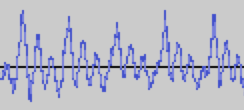
\includegraphics[scale=0.8]{exampleaudio}

\includegraphics[scale=0.5]{examplevision}
\caption{Example data pair}
\label{fig:datapair}
\end{figure}

\begin{figure*}[!t]
\centering
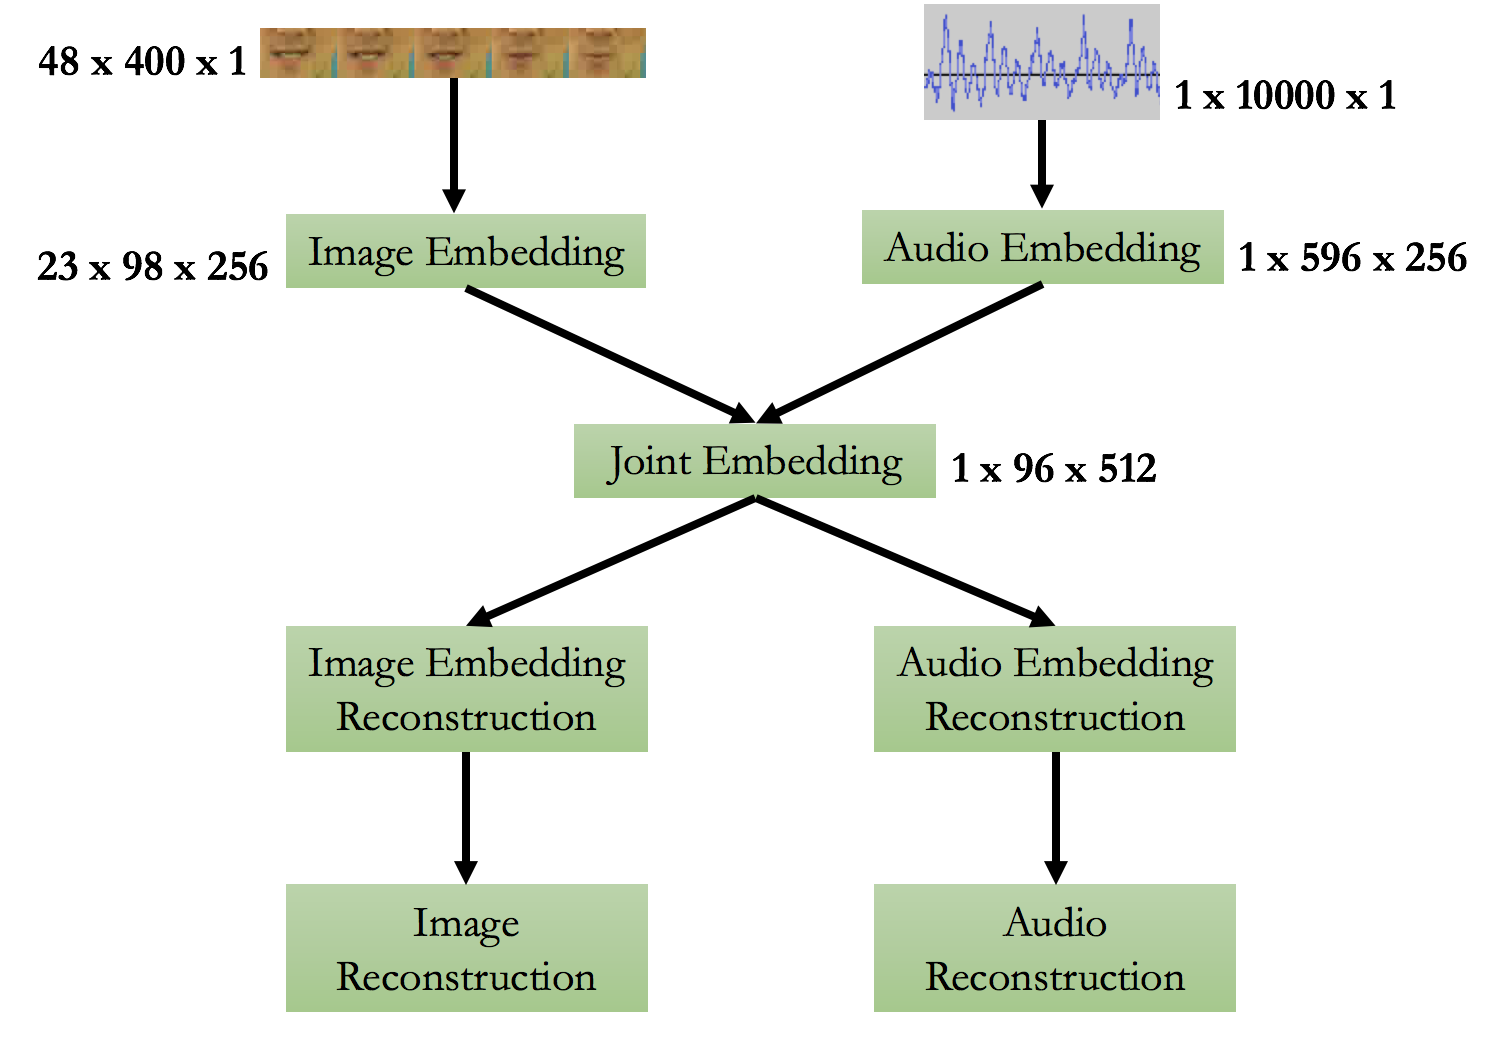
\includegraphics[scale=0.4]{standardmodel}
\caption{Multimodal Convolutional Autoencoder}
\label{fig:standardmodel}
\end{figure*}

Each video's frames are extracted as images. The videos are 3 seconds long at 25 frames per second, leading to 75 images per video. The frames contain the individual's entire head and most of their upper torso. All of the visual information that we need is produced by the mouth, so scripts are used to crop it out of each image. From here, sets of five images are concatenated together horizontally, representing 200 milliseconds of video (see Fig. \ref{fig:datapair}). Lastly, the image is converted into greyscale. The final size of the image is 400x48.

Scripts are used to separate the audio from each video, and convert it into raw wave format. The audio is sampled at 8192 kHz. The files are then segmented into 200 millisecond chunks, in order to be paired with the images. The waveform is fed into the model as a vector of size 10,000x1.

The final dataset consisted of over 400,000 data pairs. It would take too much time to train the model on the entire set, so 10,000 pairs are sampled and split into training/testing sets.

\subsection{The Model}
The model is a multimodal convolutional autoencoder (see Fig. \ref{fig:standardmodel}). 2D convolutions are used for the images, capturing both spatial and temporal features. 1D convolutions, with a large filter size, are used for the waveform. The joint embedding is created by convolving each modality down to the same size, then performing element-wise addition. The resulting embedding is then deconvolved back into an image and waveform. The model is entirely unsupervised.

The model is constructed using Keras\footnote{http://keras.io}. Each layer uses a ReLU as its activation function, the loss function is the mean squared error of the reconstructions, and the optimizer is ADADELTA.\cite{Nair2010}\cite{Zeiler2012}

\section{Results}
\subsection{Reconstruction}
The model was able to reconstruct both modalities well. A sample image reconstruction can be seen in figure \ref{fig:imgrecon}. Some detail is lost in the reconstruction, such as teeth. However, the mouth shape is preserved nicely, which is the primary feature of interest.

\begin{figure}[h]
\centering
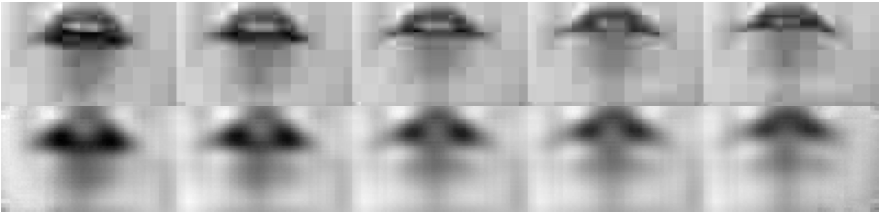
\includegraphics[scale=0.5]{imgrecon}
\caption{\textbf{Top:} Original image \textbf{Bottom:} Reconstucted Image}
\label{fig:imgrecon}
\end{figure}

\subsection{McGurk Effect}
After training, the model is fed the classic mismatched phoneme/viseme pair, /b/a and /g/a. This pair is commonly used due to the exaggerated nature of the lip movements. At this point, the image reconstruction is ignored because it has no implications for the McGurk effect. The audio reconstruction is manually evaluated to see which phoneme it most resembles. Upon evaluation, it was found that the resulting audio reconstruction did not produce an identifiable phoneme. Rather than producing a third sound, the conflicting modalities resulted in incoherent gibberish.

\begin{figure*}[!t]
\centering
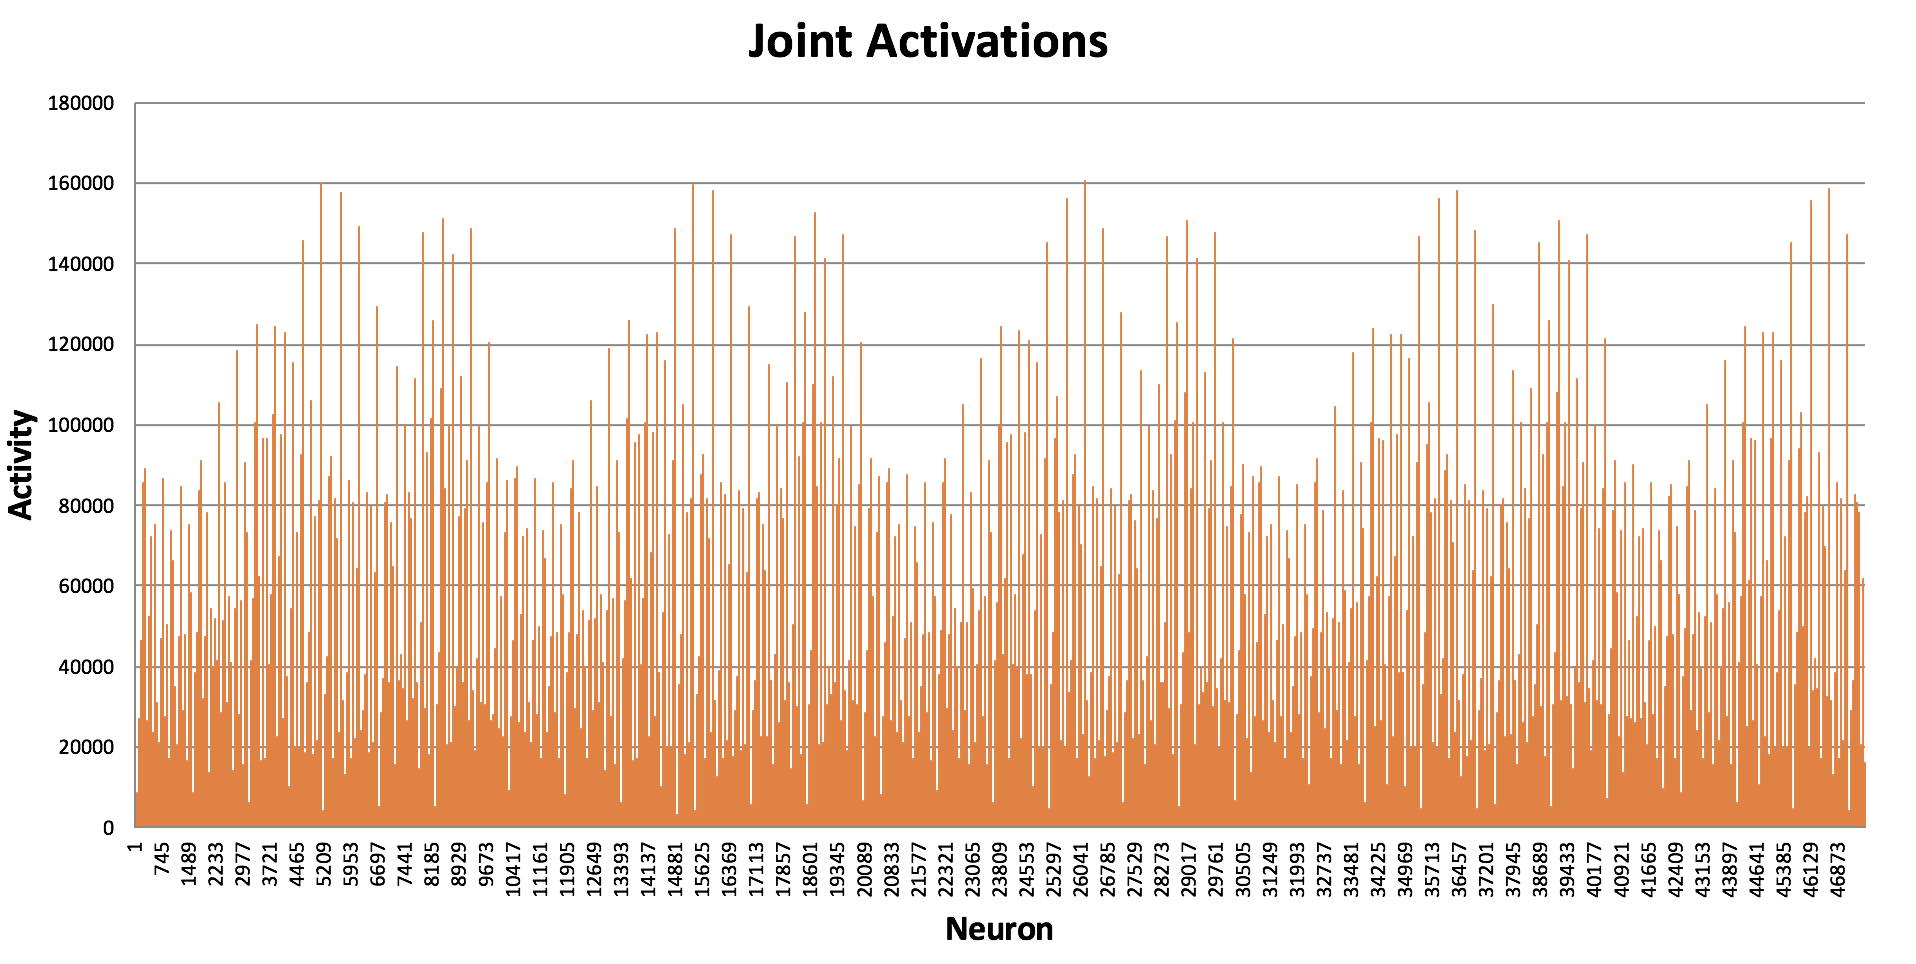
\includegraphics[scale=0.4]{sharedgraph}

\vspace{0.5cm}

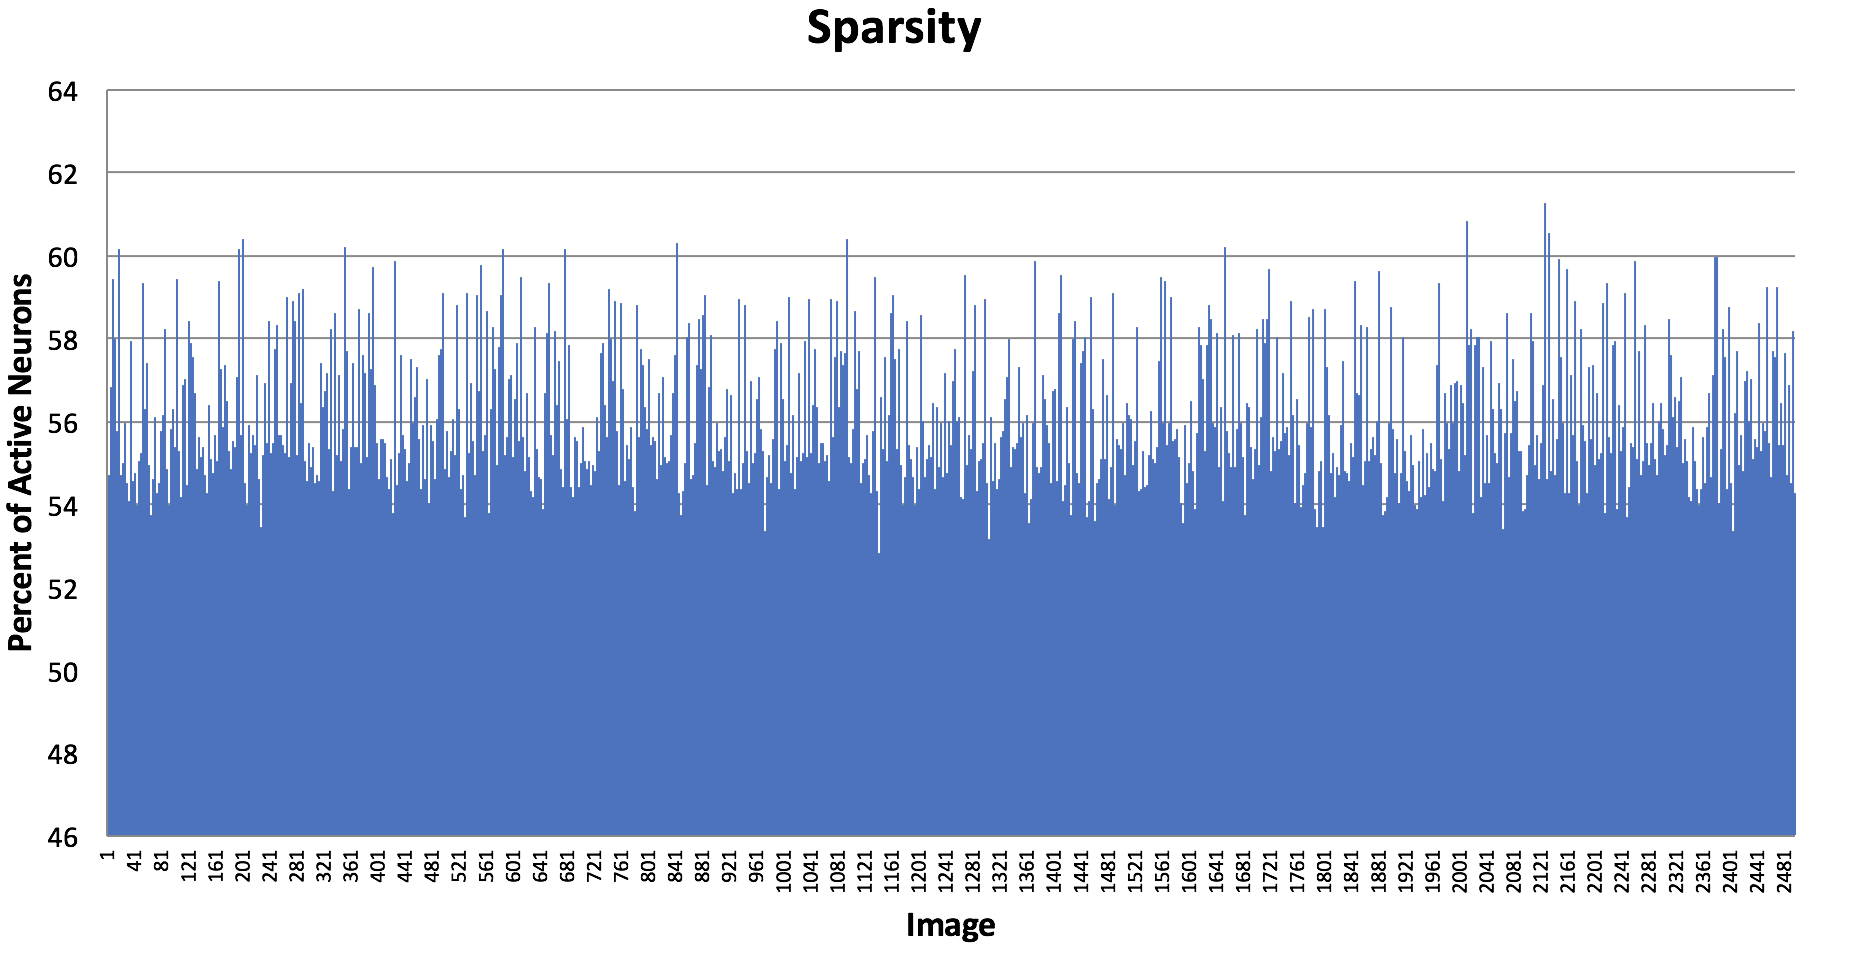
\includegraphics[scale=0.4]{sparsegraph}
\caption{\textbf{Top:} Average activation of shared neurons \textbf{Bottom:} Sparsity of embedding layer for each training image}
\label{graph:shared}
\end{figure*}

Since the model reconstructs well, the absence of the McGurk effect is most likely due to the nature of the joint embedding layer. The model must not only learn to reconstruct well, but also to align both modalities. Using the same neurons to represent common audio-visual features is the optimal way of representing data pairs in the joint layer, but finding this commonality is a difficult task. Figure \ref{graph:shared} shows the average activity for each shared neuron in the joint embedding layer. Only 35.75\% of these neurons were active for both modalities.

In order for the model to learn shared neurons, the activations of the joint layer should be sparse. If too many neurons are being used to represent the two modalities, the model will simply learn to segment embedding layer; part of the layer will be used to reconstruct the image and part will be used to reconstruct the waveform, without any shared neurons. The best way to encourage sparsity is to add normalization, such as an L1 norm, to the loss function. I attempted to add normalization to the model, but the audio reconstruction quality suffered greatly. As it stands, the model is on average 54.73\% sparse in the joint embedding layer. Figure \ref{graph:shared} displays the percentage of active neurons in the joint layer for each test data pair.

\section{Future Work}
Based upon the lack of sparsity, the model used by Kim et al. (2017) is perhaps better suited for learning the McGurk effect.\cite{Kim2017} A variation of this model for my task can be seen in figure \ref{fig:modified}. For starters, this model frames reconstruction as a hierarchical sparse coding problem. A1 sparse codes the waveform, V1 sparse codes the image, and P1 sparse codes A1 and V1. This forces the model to minimize the number of active neurons and encourages the creation of shared neurons. The model implements forms of lateral inhibition and top-down feedback. Lateral inhibition further encourages sparsity; when one neuron fires similar neurons in the layer are inhibited. Top-down feedback reinforces the interaction between the two modalities. If P1 determines that the phoneme is /d/a, it will nudge V1 and A1 into agreement. Instead of the image embedding and audio embedding competing with one another and confusing the joint layer, P1, A1, and V1 will determine the phoneme together.

\begin{figure*}[!t]
\centering
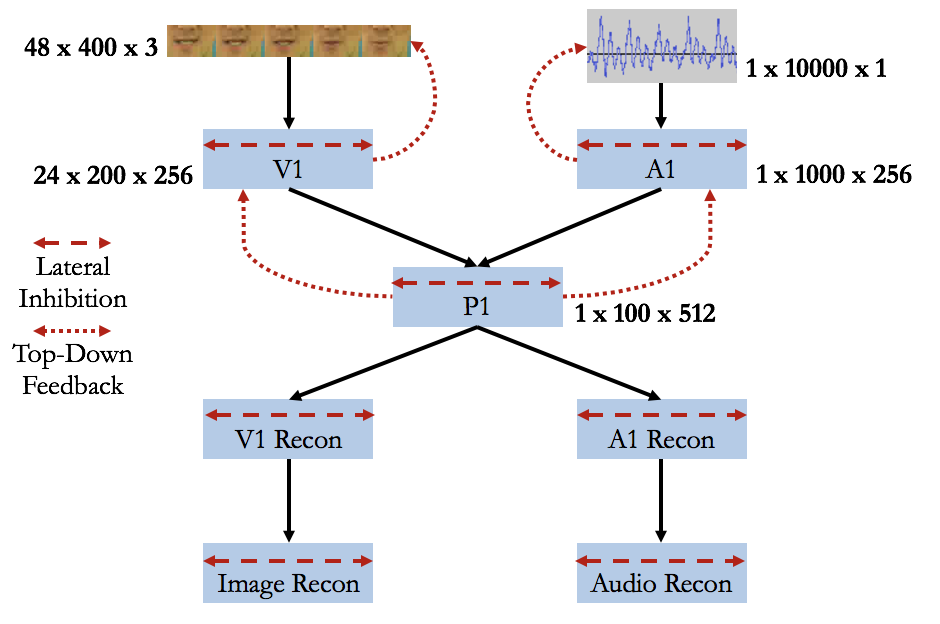
\includegraphics[scale=0.7]{modifiedmodel}
\caption{Modified Convolutional Autoencoder}
\label{fig:modified}
\end{figure*}

\section{Conclusion}
Although the model was unable to produce the McGurk effect, it led to some critical insights that suggested the model used by Kim et al. (2017) might overcome its deficiencies. This new model contains biologically inspired modifications, in the form of top-down feedback and lateral inhibition. Given the model's ability to learn specialized "Halle Berry neurons", in this context it may be able to learn specialized neurons for common phonemes. If this is indeed the case, when each modality activates the specialized neuron for its corresponding phoneme, the resulting audio reconstruction should contain the sound of both phonemes.

% trigger a \newpage just before the given reference
% number - used to balance the columns on the last page
% adjust value as needed - may need to be readjusted if
% the document is modified later
%\IEEEtriggeratref{8}
% The "triggered" command can be changed if desired:
%\IEEEtriggercmd{\enlargethispage{-5in}}

% references section

% can use a bibliography generated by BibTeX as a .bbl file
% BibTeX documentation can be easily obtained at:
% http://mirror.ctan.org/biblio/bibtex/contrib/doc/
% The IEEEtran BibTeX style support page is at:
% http://www.michaelshell.org/tex/ieeetran/bibtex/
\bibliographystyle{IEEEtran}
% argument is your BibTeX string definitions and bibliography database(s)
\bibliography{IEEEabrv,mcgurk}
%
% <OR> manually copy in the resultant .bbl file
% set second argument of \begin to the number of references
% (used to reserve space for the reference number labels box)




% that's all folks
\end{document}


